\documentclass[12pt,a4paper]{article}
\usepackage[spanish,es-tabla]{babel}
\usepackage{float}							% Insertar figuras
\usepackage{subcaption}

\usepackage[utf8]{inputenc} % Escribir con acentos, ~n...
\usepackage{eurosym} % s´ımbolo del euro
\newcommand{\horrule}[1]{\rule{\linewidth}{#1}} % Create horizontal rule command with 1 argument of height
\usepackage{listings}             % Incluye el paquete listing
\usepackage[cache=false]{minted}
\usepackage{graphics,graphicx, float} %para incluir imágenes y colocarlas
\usepackage{hyperref}
\hypersetup{
	colorlinks,
	citecolor=black,
	filecolor=black,
	linkcolor=black,
	urlcolor=black
}
\usepackage{multirow}
\usepackage{array}
\usepackage{diagbox}
\usepackage{listings}

\lstset{language=Java,
	keywordstyle=\color{RoyalBlue},
	basicstyle=\scriptsize\ttfamily,
	commentstyle=\ttfamily\itshape\color{gray},
	stringstyle=\ttfamily,
	showstringspaces=false,
	breaklines=true,
	frameround=ffff,
	frame=single,
	rulecolor=\color{black}}
\title{
\normalfont \normalsize 
\textsc{{\bf Simulación de Sistemas (2019-2020)} \\ Grado en Ingeniería Informática \\ Universidad de Granada} \\ [25pt] % Your university, school and/or department name(s)
\horrule{0.5pt} \\[0.4cm] % Thin top horizontal rule
\huge Práctica 1 \\ % The assignment title
\horrule{2pt} \\[0.5cm] % Thick bottom horizontal rule

\includegraphics{images/logo.png}	
}

\author{Antonio Jesús Heredia Castillo} % Nombre y apellidos

\date{\normalsize\today} % Incluye la fecha actual

%----------------------------------------------------------------------------------------
% DOCUMENTO
%----------------------------------------------------------------------------------------

\begin{document}

\maketitle % Muestra el Título
\newpage %inserta un salto de página
\tableofcontents % para generar el índice de contenidos
\newpage
\section{Mi Primer Modelo de Simulación de MonteCarlo}
En este simulador tenemos como variables de entrada las siguientes variables:
\begin{itemize}
	\item \textbf{Numero de iteraciones}: la cantidad de repeticiones que se va ejecutar el simulador
	\item \textbf{Posición de destino:} La posición donde quiere aparcar el usuario.
	\item \textbf{Numero de posiciones a la vista:} La cantidad de posiciones que puede ver hacia delante el conductor desde el coche.
	\item \textbf{Probabilidad de plaza ocupada: } Con que probabilidad se va a encontrar la plaza ocupada.
\end{itemize}

Dependiendo de las variables de entrada que especifiquemos tendremos unos datos de salida diferentes. \\
La primera prueba que realizaremos  es ejecutar la misma simulación varias veces para ver como afecta la la generación de numeros aleatorios.

\begin{table}[H]
	\centering
	\begin{tabular}{|l|l|l|l|}
		\hline
		\textbf{Variable entrada} & \textbf{Valor}\\ \hline
		Numero de iteraciones&100000\\ \hline
		Posición de destino&100\\ \hline
		Numero de posiciones a la vista&2\\ \hline
		Probabilidad de plaza ocupada&0.9\\ \hline
	\end{tabular}
\end{table}
Ejecutaremos varias veces la simulación con estos datos y veremos en una tabla comparativa como afecta. 
\begin{table}[H]
	\centering
	\begin{tabular}{|l|l|l|l|}
		\hline
		\textbf{Nº simulación} & \textbf{Mejor posición inicial}&\textbf{Mejor distancia}\\ \hline
		1&94&6.47\\\hline
		2&94&6.55\\\hline
		3&95&6.48\\\hline
		4&94&6.48\\\hline
		5&94&6.54\\\hline
		6&95&6.50\\\hline
	\end{tabular}

\end{table}
Como podemos ver la simulación varia muy poco en las diferentes. Esto se puede ver mejor en la Figura \ref{fig:mediadistancia}. En la que todos los valores están entre $6.4$ y $6.6$.
\begin{figure}[H]
	\centering
	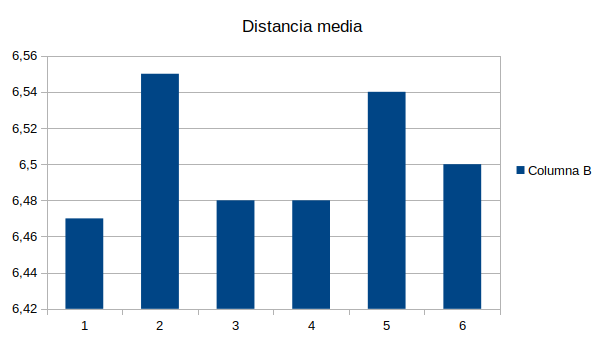
\includegraphics{images/mediaDistancia}
	\caption{Distancia media en las diferentes simulaciones.}
	\label{fig:mediadistancia}
\end{figure}
Aunque de forma intuitiva podemos ver como a pesar de tener una probabilidad muy alta de que la plaza este ocupada siempre encuentra aparcamiento a una distancia que podemos considerar cercana. Veremos si esto se cumple cambiando los parámetros de entrada y haciendo diferentes simulaciones.

\subsection{Variando la posición de destino}
Para ver si afecta la a la distancia la posición a la que se quiere ir ejecutaremos varias veces la simulación con distintas posiciones final. Aunque intuitivamente podemos pensar que no, lo comprobaremos. \\ Ejecutaremos la simulación con las siguientes variables:
\begin{table}[H]
	\centering
	\begin{tabular}{|l|l|l|l|}
		\hline
		\textbf{Variable entrada} & \textbf{Valor}\\ \hline
		Numero de iteraciones&100000\\ \hline
		Posición de destino&97:103\\ \hline
		Numero de posiciones a la vista&2\\ \hline
		Probabilidad de plaza ocupada&0.9\\ \hline
	\end{tabular}
\end{table}
En la Figura \ref{fig:distanciaPosFinal} podemos observar que lo que intuíamos se cumple. Podemos ver como la curva de disminución de la distancia media en función de la posición inicial donde comienza a buscar aparcamiento es igual pero desplazada una posición. Por lo tanto  en vista de los resultados podemos confirmar que la posición final no afecta a la mejor distancia para encontrar aparcamiento.
\begin{figure}[H]
	\centering
	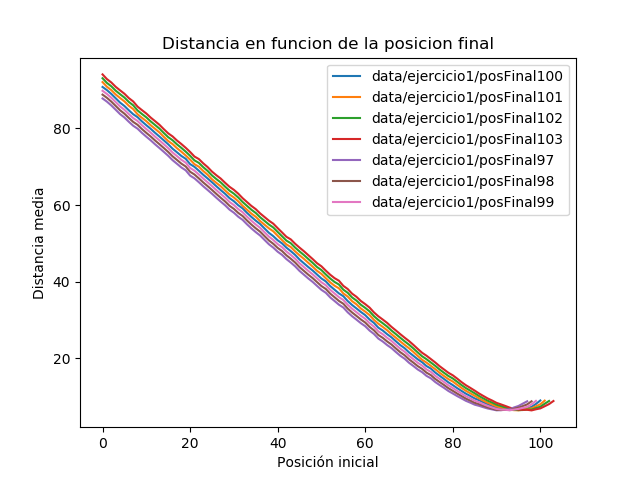
\includegraphics{images/distanciaPosFinal.png}
	\caption{Distancia media en relación a la posición final.}
	\label{fig:distanciaPosFinal}
\end{figure}
\subsection{Variando el numero de posiciones a la vista}
En este caso podemos pensar que cuantas mas posiciones ves hacia delante mejor podrás  predecir cuando escoger un aparcamiento y cuando no y asi mejorar la distancia a la que aparcar. Veremos si se cumple o en clase de que se cumpla si merece la pena anticiparse.\\
En este caso ejecutaremos la simulación con las siguientes variables:
\begin{table}[H]
	\centering
	\begin{tabular}{|l|l|l|l|}
		\hline
		\textbf{Variable entrada} & \textbf{Valor}\\ \hline
		Numero de iteraciones&100000\\ \hline
		Posición de destino&100\\ \hline
		Numero de posiciones a la vista&2,12,22,32\\ \hline
		Probabilidad de plaza ocupada&0.9\\ \hline
	\end{tabular}
\end{table}
Para analizar los datos usaremos la Figura \ref{fig:distanciaVisibilidad} que la visualizaremos en tres dimensiones, aunque no nos importa mucho en que posición inicial empezamos a buscar aparcamiento. Como podemos ver con visibilidad $0$  la distancia de aparcado esta entorno a $6.5$ y conforme aumentamos la visibilidad disminuye fuertemente. hasta que llega entorno al $4.75$ y ya apenas varia. Con estos datos podemos deducir que cuanto mas coches hacia delante intente ver el conductor mas cerca podra aparcar de su destino. 
\begin{figure}[H]
	\centering
	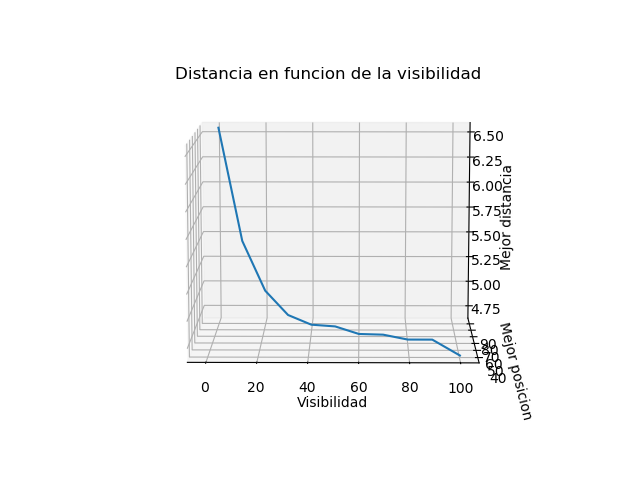
\includegraphics{images/distanciaVisivilidad.png}
	\caption{Distancia media en relación a la visibilidad final.}
	\label{fig:distanciaVisibilidad}
\end{figure}
\subsection{Variando la probabilidad de plaza ocupada}
En este caso cambiaremos la probabilidad en que una plaza este libre o no. Como es de esperar cuanto mas probable sea que la plaza este ocupada mas difícil sera encontrar aparcamiento y por ende mas lejos se tendrá que aparcar.\\La simulación la he realizado con los siguientes datos.
\begin{table}[H]
	\centering
	\begin{tabular}{|l|l|l|l|}
		\hline
		\textbf{Variable entrada} & \textbf{Valor}\\ \hline
		Numero de iteraciones&100000\\ \hline
		Posición de destino&100\\ \hline
		Numero de posiciones a la vista&2\\ \hline
		Probabilidad de plaza ocupada&0.5,0.6,...,0.9\\ \hline
	\end{tabular}
\end{table}
Según la Figura \ref{fig:distProbabilidad} podemos observar que la distancia en función de la probabilidad de que este ocupada tiene un crecimiento exponencial y afecta mucho a la hora tener una distancia mejor o peor. 
\begin{figure}[H]
	\centering
	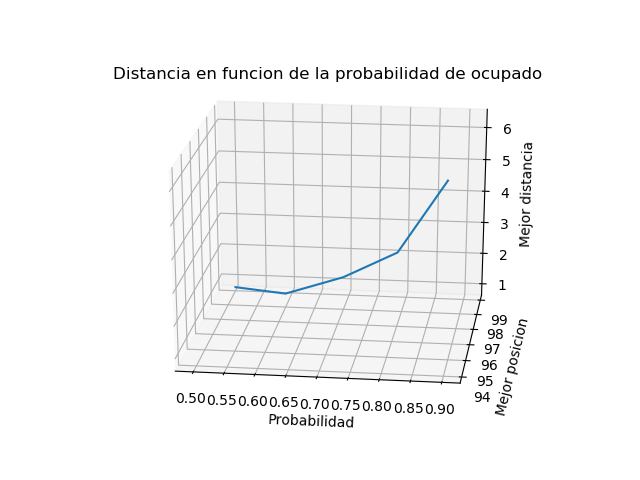
\includegraphics{images/probabilidad.png}
	\caption{Distancia media en relación a la visibilidad final.}
	\label{fig:distProbabilidad}
\end{figure}
En cambio la distancia a la que deberíamos empezar a buscar aparcamiento si que varia de forma linea como podemos ver en la Figura \ref{fig:distProbabilidad2}.
\begin{figure}[H]
	\centering
	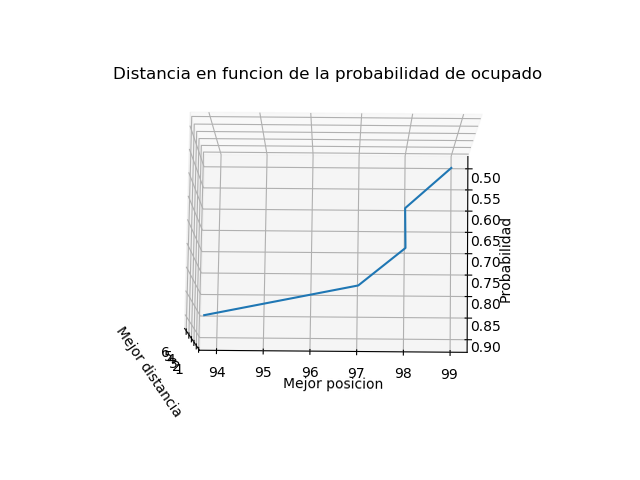
\includegraphics{images/prob2.png}
	\caption{Distancia media en relación a la visibilidad final.}
	\label{fig:distProbabilidad2}
\end{figure}
Si nos pusieramos en el caso de que fuera imposible encontrar aparcamiento porque todas las plazas van a estar llenas el simulador fallaría como podemos ver la Figura \ref{fig:falloej1}.
\begin{figure}[H]
	\centering
	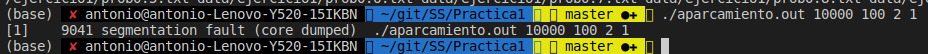
\includegraphics[width=0.7\linewidth]{images/falloej1}
	\caption{}
	\label{fig:falloej1}
\end{figure}
\section{Mi primer Modelo de Simulación Discreto}
\subsection{Numero de repuestos minimos}
En esta simulación vamos a obtener datos del tiempo en el que vamos a estar desprotegidos (sin radares). Para ver cual seria el mínimo numero de repuestos que podemos tener para no estar desprotegidos en ningún momento. La simulación con distinto numero de respuestos las vamos a ejecutar 5, 50, 500 y 5000 veces. En la siguiente tabla podemos ver los datos.
\begin{tabular}{|l|l|l|l|l|}
	\hline 
	Nº de repuestos & Nº de repeticiones & Media de fallos & Porcentaje tiempo desprotección \\ 
	\hline 
		\hline 
	3 & 5 & 55.4 & 69.33  \\ 
	3 & 50 & 52.54 & 64.3059   \\ 
	3 & 500 & 53.09 & 65.5727  \\ 
	3 & 5000 &  52.90 & 65.472  \\ 
	\hline 
		\hline
	5 & 5 & 41& 36.24  \\ 
	5 & 50 & 42.02 & 37.77   \\ 
	5 & 500 & 39.91 & 36.4588  \\ 
	5 & 5000 &  40.25 & 36.97  \\ 
	\hline 
		\hline
	8 & 5 & 8& 5.98  \\ 
	8 & 50 & 13.34 & 8.95   \\ 
	8 & 500 & 13.69 & 8.79  \\ 
	8 & 5000 &  13.71 & 8.87  \\ 
	\hline
	\hline
	11 & 5 & 2& 0.59  \\ 
	11 & 50 & 1.62 & 0.78   \\ 
	11 & 500 & 1.91 & 0.95  \\ 
	11 & 5000 &  2.0862 & 1.02 \\ 
	\hline
	\hline
		12 & 5 & 0& 0  \\ 
	12 & 50 & 0.9 & 0.3   \\ 
	12 & 500 & 0.788 & 0.36  \\ 
	12 & 5000 &  0.85 & 0.40 \\ 
	 
	\hline   
	\hline
	16 & 5 & 0& 0  \\ 
	16 & 50 & 0 & 0   \\ 
	16 & 500 & 0.024 & 0.011  \\ 
	16 & 5000 &  0.019 & 0.00559 \\
	\hline 
\end{tabular}
De estos estos datos podemos sacar varias conclusiones. La primera es que al simular mas veces obtenemos resultados mas consistentes. Cuando lo ejecutas varias veces con una sola repetición los datos medios (en ese caso los datos a secas) obtenidos son muy dispares en las distintas ejecuciones. Esto se debe principalmente a las variables aleatorias que afectan a la propia simulación. Por otro lado podemos ver como aunque es cierto que a mayor cantidad de repuestos menos \% de tiempo sin protección tenemos, llega un momento en el que no merece la pena tener mas. Para mi en mi, en las simulaciones realizadas esa cantidad es de \textbf{12}. \\ Como podemos ver en la cantidad 12 es cuando el porcentaje de tiempo desprotegidos baja del cero por ciento y la diferencia entre tener 12 o 16 no son excesivamente significativas.
\subsection{Otros experimentos}
\subsection{Tiempo de vida}
Para este ejemplo lo que haremos es usar el tiempo de vida por defecto, uno menor y otro mayor, para si necesitamos mas piezas de repuesto o las mimas, para que tener un porcentaje de tiempo de desproteción menor al 1\%.
\begin{tabular}{|c|c|c|c|}
	\hline 
	Tiempo de vida & Nº repuestos & Nº fallos & Porcentaje tiempo desproteción \\ 
	\hline  
	\hline
 	5& 5 &128.743 & 95.99 \\  
	20&5 &39.95 & 36.83 \\ 
	70& 5& 0.51 & 0.49 \\ 	
	\hline
	\hline  
	5& 12 &178.43 & 76.71 \\ 
	20&12 &0.871 & 0.4122 \\ 
	70& 12 & 0 & 0 \\ 
	\hline
	\hline  
	5& 30 &15.3 & 2.95 \\ 
	20&30 &0 & 0 \\ 
	70& 30& 0  & 0  \\ 
	\hline   
\end{tabular} 
Como podemos ver la vida útil en los componentes de los radares son un factor muy importante para que el tiempo de desproteción sea minimo. Si fuéramos el ``ministerio de defensa'' de algún país podríamos intentar optimizar la cantidad de repuesto que tenemos frente a la vida útil de los mismos para ahorrar costes teniendo el mismo porcentaje de desproteción. 
\subsection{Tiempo de reparación}
Ahora realizaremos experimentos con diferentes tiempos de reparación mínimos y máximos para ver como afecta esta variabilidad pero sin cambiar el numero de repuestos ni la vida útil, que en este caso serán siete y veinte respectivamente.\\\\
\begin{tabular}{|c|c|c|c|}
	\hline 
	vmin & vmax & Nº fallos &Porcentaje tiempo desproteción \\ 
	\hline 	
	5 &15 & 1.47  & 0.38 \\
	5 &30 & 10.55  & 6.001 \\
	5 &45 & 26.28  & 20.90 \\ 
		\hline 		\hline 	   
	10 &15 & 2.96  & 1.22 \\ 
	10 &30 & 16.221  & 10.47 \\ 
	10 &45 & 30.645  & 26.71 \\ 
	\hline
	\hline 	   
	15 &15 & 6.29  & 3.10 \\ 
	15 &30 & 21.22  & 15.31 \\ 
	15 &45 & 34.99  & 33.03 \\ 
	\hline  
\end{tabular} 
\\\\
Como podemos ver el tiempo  que tardan en reparar los radares tambien afecta mucho en el porcentaje de tiempo sin proteción. Para la misma cantidad de respuestos cuanto menos tarden en arreglar el radar menos tiempo estaremos sin su servicio. Por lo tanto a lo mejor convendría invertir mas en tener técnicos de reparación antes que tener muchos repuestos con el gasto en almacén que eso supondría. 
\section{Mi primer Modelo de Simulación Continuo}
\end{document}
	